\documentclass{article}%
\usepackage[T1]{fontenc}%
\usepackage[utf8]{inputenc}%
\usepackage{lmodern}%
\usepackage{textcomp}%
\usepackage{lastpage}%
\usepackage{geometry}%
\geometry{tmargin=2cm,rmargin=2.5cm,lmargin=2.5cm}%
\usepackage{ragged2e}%
\usepackage{booktabs}%
\usepackage{multirow}%
\usepackage{enumitem}%
\usepackage{graphicx}%
%
\usepackage{graphicx}%
\usepackage{graphicx}%
\usepackage{float}%
%
\begin{document}%
\normalsize%
\begin{minipage}{\textwidth}%
\centering%
\begin{Large}%
Relatório das Redes Sociais e Portal%
\end{Large}%
\linebreak%
\linebreak%
\linebreak%
\begin{large}%
Fevereiro de 2024%
\end{large}%
\linebreak%
\end{minipage}%
\section*{Tribuna do Norte}%
\label{sec:TribunadoNorte}%
\subsection*{Resultados de janeiro/2024}%
\label{subsec:Resultadosdejaneiro/2024}%
\begin{minipage}{\textwidth}%
\centering%
\begin{tabular}{@{}|c|c|c|c|@{}}%
\toprule%
\multirow{2}{*}{Portal}&0&0&0\\%
&novos usuários&visualizações&usuários recorrentes\\%
\midrule%
\multirow{2}{*}{Instagram}&{-}529.865&0&151.885\\%
&novos seguidores&contas atingidas&visitas ao perfil\\%
\midrule%
\multirow{2}{*}{Facebook}&{-}332.603&0&0\\%
&novos seguidores&contas atingidas&visitas ao perfil\\%
\midrule%
\multirow{2}{*}{Twitter}&{-}311.129&0&0\\%
&novos seguidores&impressões&engajamentos\\%
\midrule%
\multirow{2}{*}{Youtube}&{-}34.000&0&0\\%
&novos inscritos&visualizações&horas de exibição\\\bottomrule%
%
\end{tabular}%
\end{minipage}%
\begin{itemize}%
\item%
Ao todo, a Tribuna do Norte entregou seu conteúdo para, aproximadamente, 829.760 novas contas, entre Portal, Instagram, Twitter, Facebook e YouTube.%
\item%
\textbf{Instagram}%
\begin{enumerate}[label=-]%
\item%
Total de seguidores atual: 0. Total de seguidores no mês anterior: 529.865%
\item%
Seguidores adquiridos no mês: {-}529.865. Deixaram de seguir: 0.%
\item%
Taxa de fixação: 100,0\%%
\end{enumerate}%
\item%
\textbf{Facebook}%
\begin{enumerate}[label=-]%
\item%
Total de seguidores atual: 0. Total de seguidores no mês anterior: 332.603%
\item%
Seguidores adquiridos no mês: {-}332.603. Deixaram de seguir: 0.%
\item%
Taxa de fixação: 100,0\%%
\end{enumerate}%
\item%
\textbf{Twitter}%
\begin{enumerate}[label=-]%
\item%
Total de seguidores atual: 0. Total de seguidores no mês anterior: 311.129%
\item%
Seguidores adquiridos no mês: {-}311.129. Deixaram de seguir: 0.%
\item%
Taxa de fixação: 100,0\%%
\end{enumerate}%
\item%
\textbf{YouTube}%
\begin{enumerate}[label=-]%
\item%
Total de seguidores atual: 0. Total de seguidores no mês anterior: 34.000%
\item%
Seguidores adquiridos no mês: {-}34.000. Deixaram de seguir: 0%
\item%
Taxa de fixação: 100,0\%%
\end{enumerate}%
\end{itemize}

%
\newpage%
\subsection*{Análise mensal}%
\label{subsec:Anlisemensal}%
\subsubsection*{Portal}%
\label{ssubsec:Portal}%
\begin{minipage}{\textwidth}%
\centering%
\begin{tabular}{@{}|c|c|c|c|@{}}%
\toprule%
\multirow{3}{*}{Mês}&Novos usuários&Visualizações&Usuários recorrentes\\%
&\begin{footnotesize}%
variação em relação ao%
\end{footnotesize}&\begin{footnotesize}%
variação em relação ao%
\end{footnotesize}&\begin{footnotesize}%
variação em relação ao%
\end{footnotesize}\\%
&\begin{footnotesize}%
mês anterior | mesmo mês em 2023%
\end{footnotesize}&\begin{footnotesize}%
mês anterior | mesmo mês em 2023%
\end{footnotesize}&\begin{footnotesize}%
mês anterior | mesmo mês em 2023%
\end{footnotesize}\\%
\midrule%
\multirow{2}{*}{Janeiro}&819 mil&3,5 milhões&279 mil\\%
&\begin{footnotesize}%
+2\% | +29\%%
\end{footnotesize}&\begin{footnotesize}%
+13\% | {-}30\%%
\end{footnotesize}&\begin{footnotesize}%
{-}3,5\% | +37,4\%%
\end{footnotesize}\\%
\midrule%
\multirow{2}{*}{Fevereiro}&('0', 0) &('0', 0) &('0', 0) \\%
&\begin{footnotesize}%
{-}100,0\% | {-}100,0\%%
\end{footnotesize}&\begin{footnotesize}%
{-}100,0\% | {-}100,0\%%
\end{footnotesize}&\begin{footnotesize}%
{-}100,0\% | {-}100,0\%%
\end{footnotesize}\\\bottomrule%
%
\end{tabular}%
\end{minipage}

%
\subsection*{}%
\label{subsec:}%
Portal: origem dos usuários%


\begin{figure}[H]%
\centering%
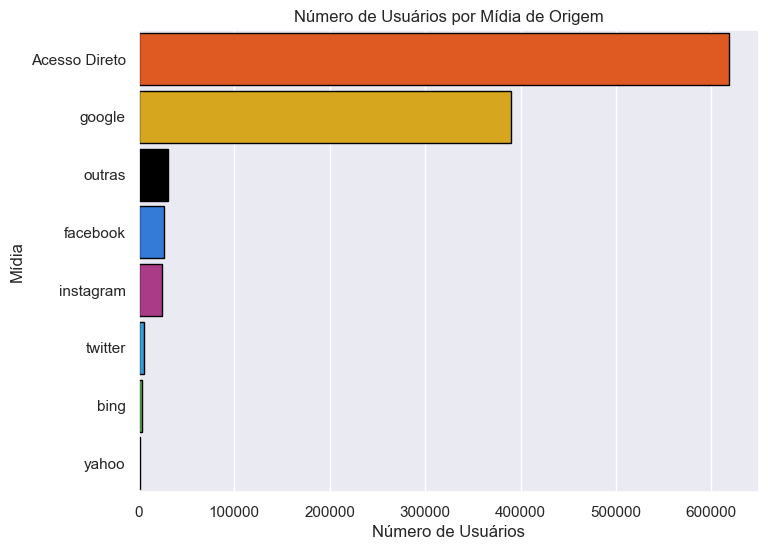
\includegraphics[width=1\textwidth]{C:/Users/Usuario/Desktop/Nova pasta/origem.png}%
\end{figure}

%
\newpage%
\subsection*{}%
\label{subsec:}%
Portal: 10 notícias mais vistas%


\begin{figure}[H]%
\centering%
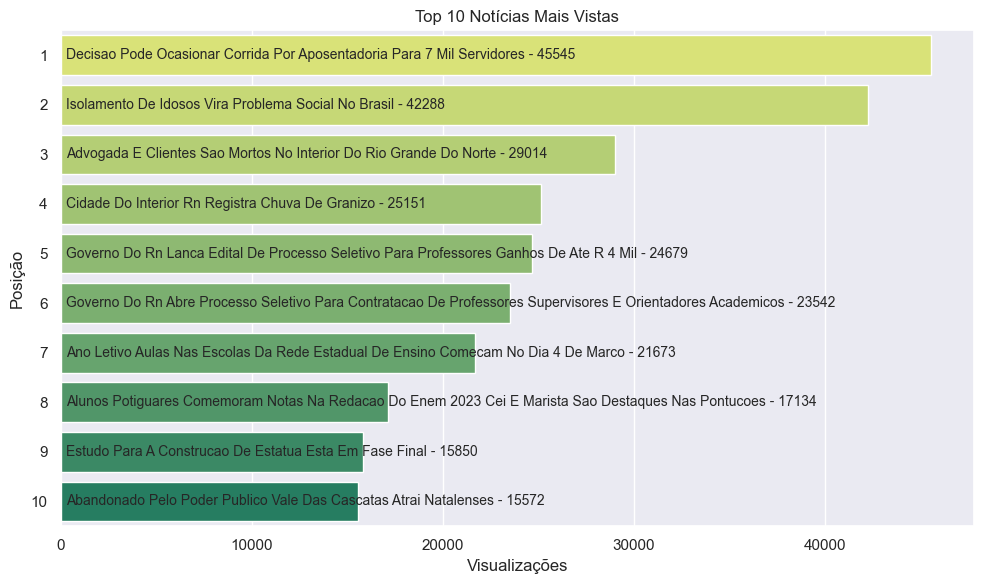
\includegraphics[width=0.8\textwidth]{C:/Users/Usuario/Desktop/Nova pasta/top10.png}%
\end{figure}

%
\subsection*{}%
\label{subsec:}%
Portal: 15 notícias mais pesquisadas%


\begin{figure}[H]%
\centering%
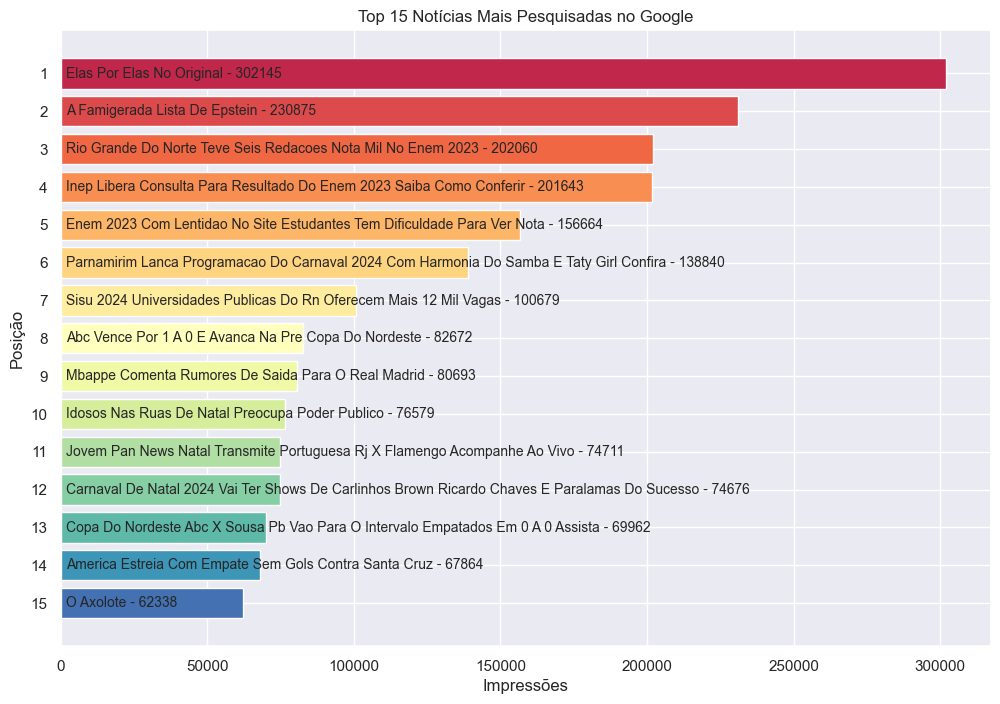
\includegraphics[width=0.9\textwidth]{C:/Users/Usuario/Desktop/Nova pasta/top15.png}%
\end{figure}

%
\subsection*{}%
\label{subsec:}%
Portal: comparativo de visualizações e acessos de usuários%


\begin{figure}[H]%
\centering%
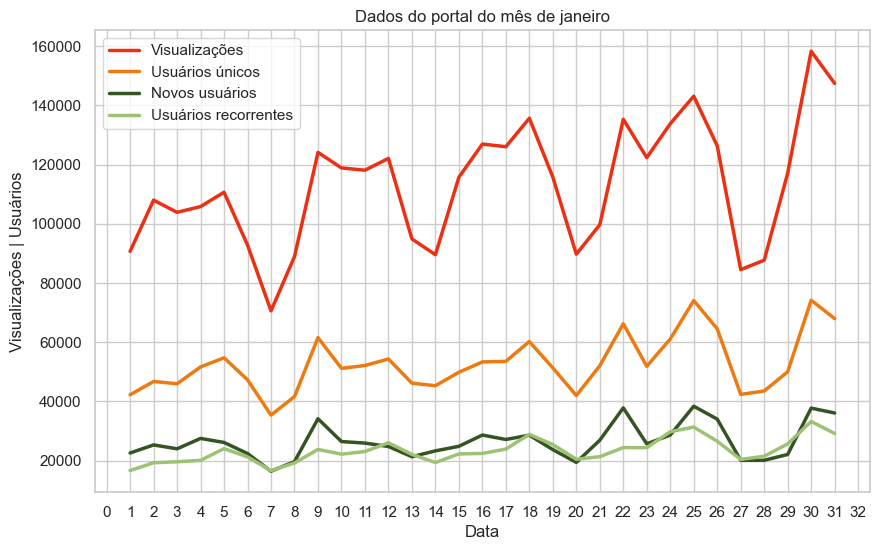
\includegraphics[width=0.8\textwidth]{C:/Users/Usuario/Desktop/Nova pasta/visualizacoesUsuarios.png}%
\end{figure}

%
\subsection*{}%
\label{subsec:}%
Portal: visualizações por faixa etária%


\begin{figure}[H]%
\centering%
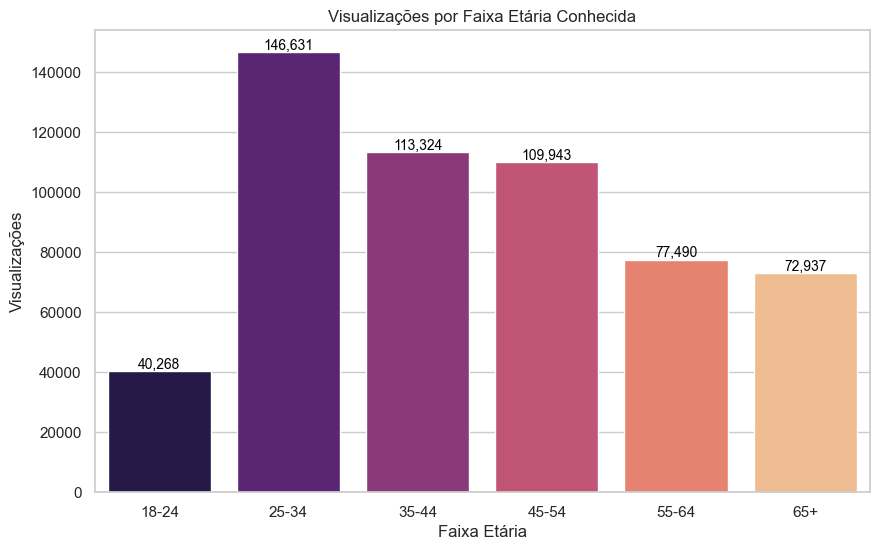
\includegraphics[width=0.8\textwidth]{C:/Users/Usuario/Desktop/Nova pasta/faixaEtaria.png}%
\end{figure}

%
\newpage%
\section*{}%
\label{sec:}%
Portal: visualizações por faixa etária (desconhecida e total)%


\begin{figure}[H]%
\centering%
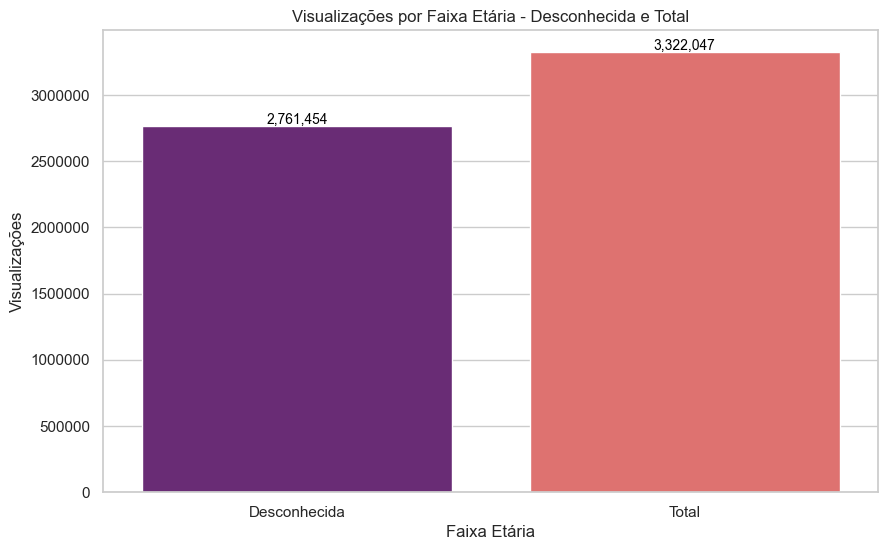
\includegraphics[width=0.8\textwidth]{C:/Users/Usuario/Desktop/Nova pasta/faixaEtaria_desconhecidaAndTotal.png}%
\end{figure}

%
\newpage%
\subsection*{Análise mensal}%
\label{subsec:Anlisemensal}%
\subsubsection*{Instagram}%
\label{ssubsec:Instagram}%
\begin{minipage}{\textwidth}%
\centering%
\begin{tabular}{@{}|c|c|c|c|@{}}%
\toprule%
\multirow{3}{*}{Mês}&Novos seguidores&Alcance&Visitas\\%
&\begin{footnotesize}%
variação em relação ao%
\end{footnotesize}&\begin{footnotesize}%
variação em relação ao%
\end{footnotesize}&\begin{footnotesize}%
variação em relação ao%
\end{footnotesize}\\%
&\begin{footnotesize}%
mês anterior | mesmo mês em 2023%
\end{footnotesize}&\begin{footnotesize}%
mês anterior | mesmo mês em 2023%
\end{footnotesize}&\begin{footnotesize}%
mês anterior | mesmo mês em 2023%
\end{footnotesize}\\%
\midrule%
\multirow{2}{*}{Janeiro}&6,7 mil&542 mil&152 mil\\%
&\begin{footnotesize}%
+21,8\% | +440,3\%%
\end{footnotesize}&\begin{footnotesize}%
{-}7\% | {-}19\%%
\end{footnotesize}&\begin{footnotesize}%
+17,2\% | {-}26,2\%%
\end{footnotesize}\\%
\midrule%
\multirow{2}{*}{Fevereiro}&('0', 0) &('0', 0) &('0', 0) \\%
&\begin{footnotesize}%
{-}100,0\% | {-}100,0\%%
\end{footnotesize}&\begin{footnotesize}%
{-}100,0\% | {-}100,0\%%
\end{footnotesize}&\begin{footnotesize}%
{-}100,0\% | {-}100,0\%%
\end{footnotesize}\\\bottomrule%
%
\end{tabular}%
\end{minipage}%
\begin{itemize}%
\item%
Legenda:%
\begin{enumerate}[label=-]%
\item%
\textbf{Alcance:} Essa métrica calcula o alcance da distribuição orgânica ou paga do seu conteúdo do Instagram e/ou Facebook, incluindo publicações e stories que foram turbinados. Também pode ser interpretada como a quantidade de contas atingidas;%
\item%
\textbf{Visitas:} número de vezes que usuários visitaram seu perfil.%
\end{enumerate}%
\end{itemize}

%
\subsection*{Análise mensal}%
\label{subsec:Anlisemensal}%
\subsubsection*{Facebook}%
\label{ssubsec:Facebook}%
\begin{minipage}{\textwidth}%
\centering%
\begin{tabular}{@{}|c|c|c|c|@{}}%
\toprule%
\multirow{3}{*}{Mês}&Novos seguidores&Alcance&Visitas\\%
&\begin{footnotesize}%
variação em relação ao%
\end{footnotesize}&\begin{footnotesize}%
variação em relação ao%
\end{footnotesize}&\begin{footnotesize}%
variação em relação ao%
\end{footnotesize}\\%
&\begin{footnotesize}%
mês anterior | mesmo mês em 2023%
\end{footnotesize}&\begin{footnotesize}%
mês anterior | mesmo mês em 2023%
\end{footnotesize}&\begin{footnotesize}%
mês anterior | mesmo mês em 2023%
\end{footnotesize}\\%
\midrule%
\multirow{2}{*}{Janeiro}&628&468 mil&32 mil\\%
&\begin{footnotesize}%
+38\% | +20\%%
\end{footnotesize}&\begin{footnotesize}%
{-}5\% | {-}7,5\%%
\end{footnotesize}&\begin{footnotesize}%
+9,6\% | +4,2\%%
\end{footnotesize}\\%
\midrule%
\multirow{2}{*}{Fevereiro}&('0', 0) &('0', 0) &('0', 0) \\%
&\begin{footnotesize}%
{-}100,0\% | {-}100,0\%%
\end{footnotesize}&\begin{footnotesize}%
{-}100,0\% | {-}100,0\%%
\end{footnotesize}&\begin{footnotesize}%
{-}100,0\% | {-}100,0\%%
\end{footnotesize}\\\bottomrule%
%
\end{tabular}%
\end{minipage}%
\begin{itemize}%
\item%
Legenda:%
\begin{enumerate}[label=-]%
\item%
\textbf{Alcance:} Essa métrica calcula o alcance da distribuição orgânica ou paga do seu conteúdo do Instagram e/ou Facebook, incluindo publicações e stories que foram turbinados. Também pode ser interpretada como a quantidade de contas atingidas;%
\item%
\textbf{Visitas:} número de vezes que usuários visitaram seu perfil.%
\end{enumerate}%
\end{itemize}

%
\newpage%
\section*{}%
\label{sec:}%
FB e IG: audiência por sexo e faixa etária%


\begin{figure}[H]%
\centering%
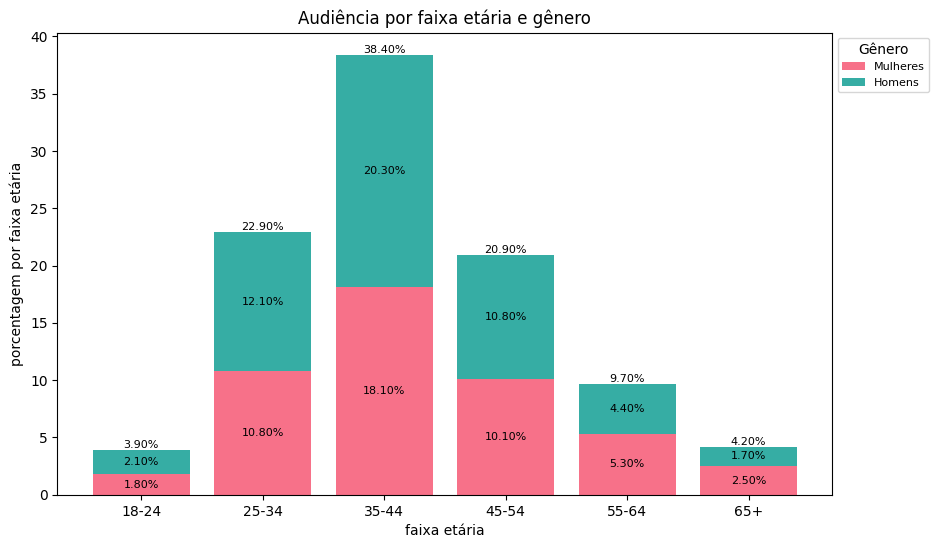
\includegraphics[width=0.8\textwidth]{C:/Users/Usuario/Desktop/Nova pasta/fePublico_FBIG.png}%
\end{figure}

%
\section*{}%
\label{sec:}%
FB e IG: audiência por cidades%


\begin{figure}[H]%
\centering%
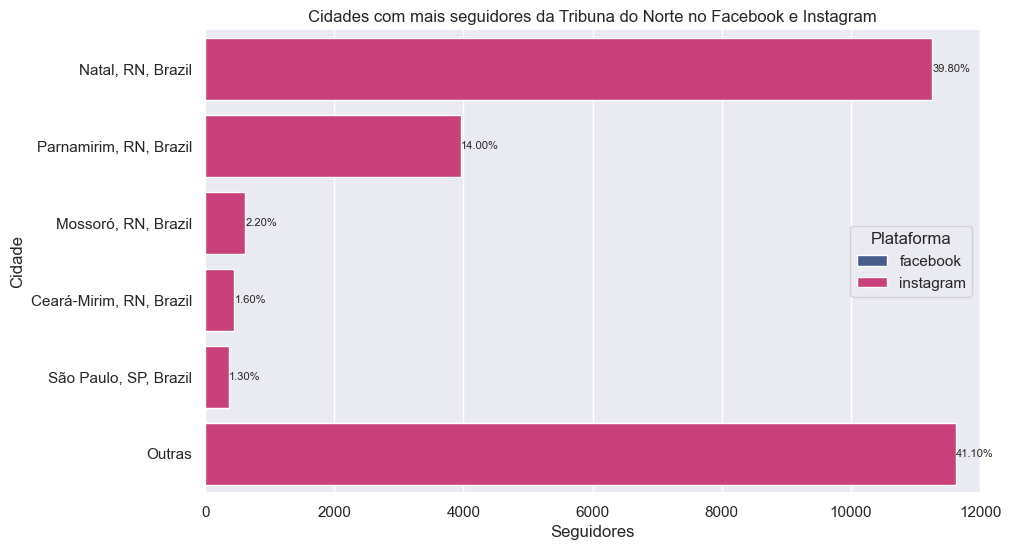
\includegraphics[width=0.8\textwidth]{C:/Users/Usuario/Desktop/Nova pasta/publicoCidades.png}%
\end{figure}

%
\newpage%
\section*{}%
\label{sec:}%
FB: visitas ao longo do mês%


\begin{figure}[H]%
\centering%
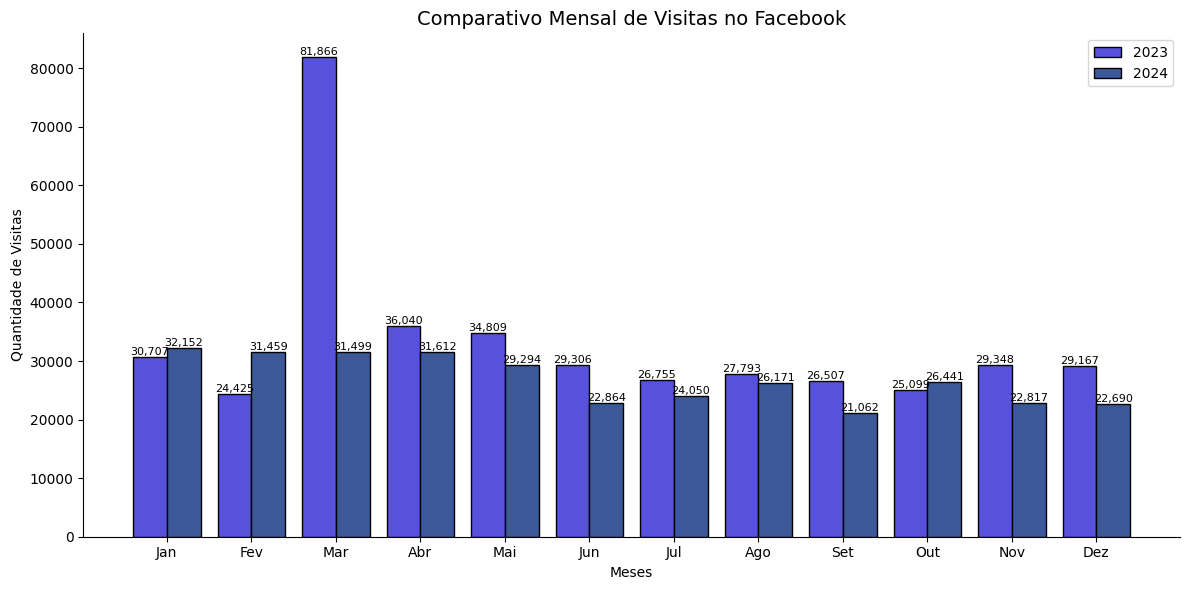
\includegraphics[width=0.75\textwidth]{C:/Users/Usuario/Desktop/Nova pasta/visitasFB.png}%
\end{figure}

%
\section*{}%
\label{sec:}%
FB: alcance ao longo do mês%


\begin{figure}[H]%
\centering%
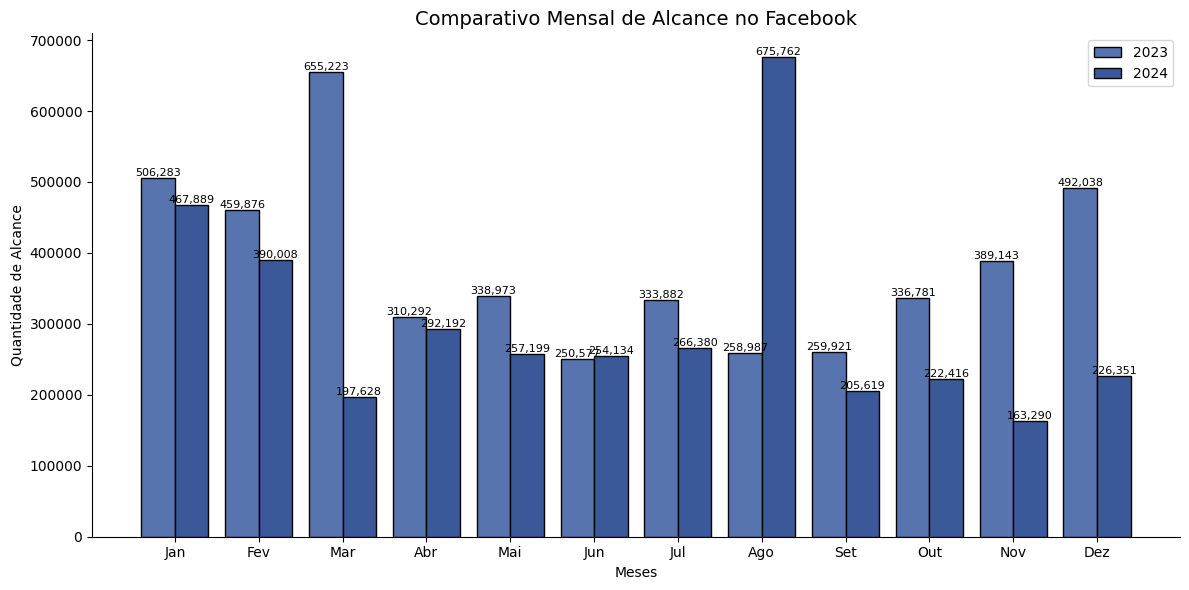
\includegraphics[width=0.75\textwidth]{C:/Users/Usuario/Desktop/Nova pasta/alcanceFB.png}%
\end{figure}

%
\section*{}%
\label{sec:}%
IG: ganho de seguidores ao longo do mês%


\begin{figure}[H]%
\centering%
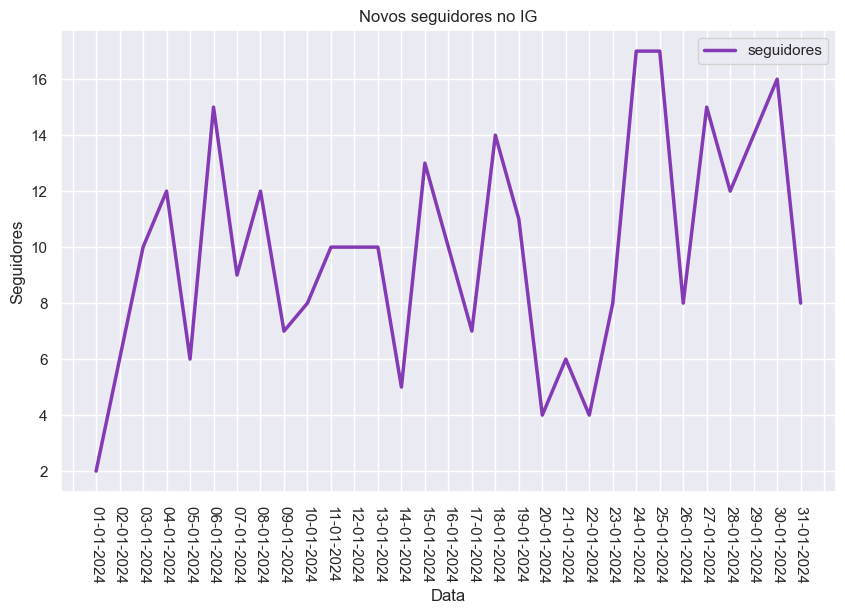
\includegraphics[width=0.45\textwidth]{C:/Users/Usuario/Desktop/Nova pasta/seguidoresIG.png}%
\end{figure}

%
\section*{}%
\label{sec:}%
IG: visitas ao perfil ao longo do mês%


\begin{figure}[H]%
\centering%
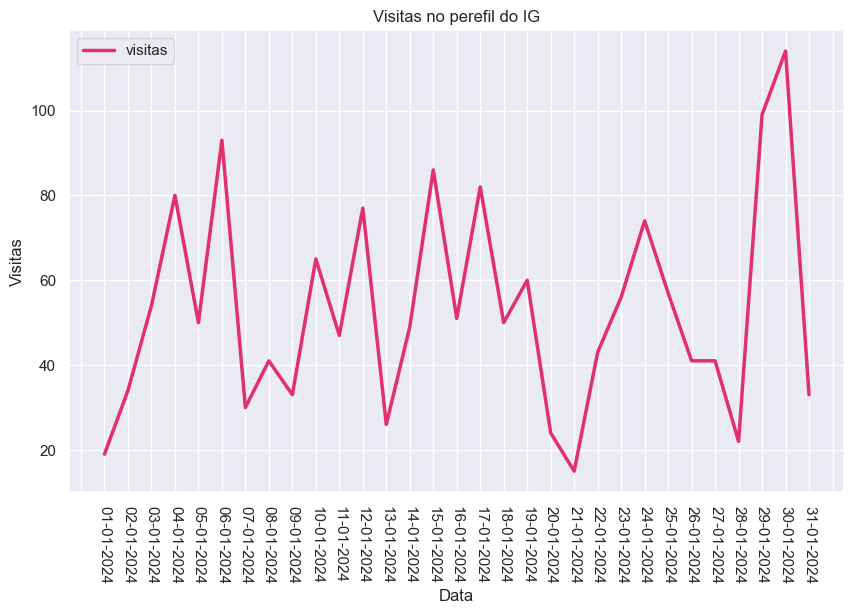
\includegraphics[width=0.45\textwidth]{C:/Users/Usuario/Desktop/Nova pasta/visitasIG.png}%
\end{figure}

%
\section*{}%
\label{sec:}%
IG: alcance do perfil ao longo do mês%


\begin{figure}[H]%
\centering%
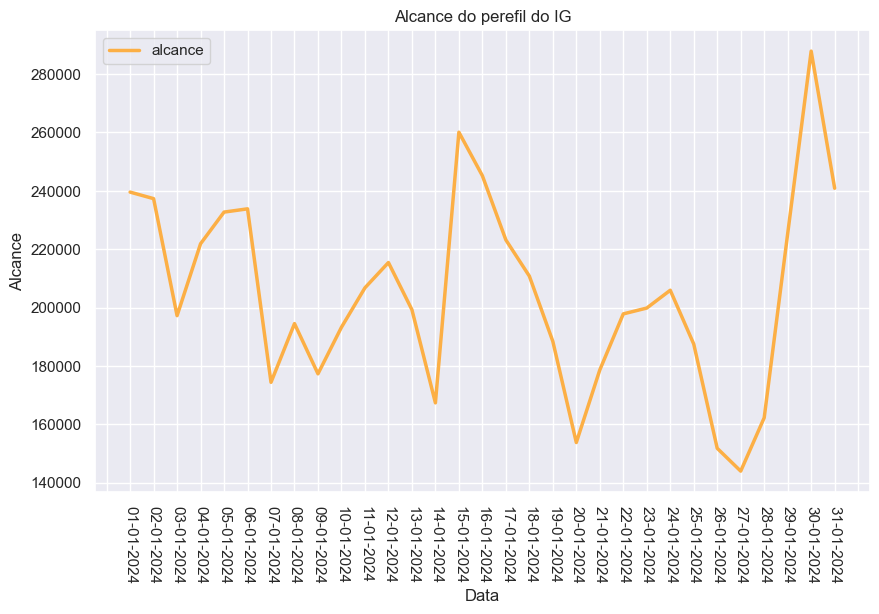
\includegraphics[width=0.45\textwidth]{C:/Users/Usuario/Desktop/Nova pasta/alcanceIG.png}%
\end{figure}

%
\newpage%
\section*{}%
\label{sec:}%
IG: comparativo de seguidores, visitas e alcance. (Obs.: dados fora de escala para uma melhor visualização)%


\begin{figure}[H]%
\centering%
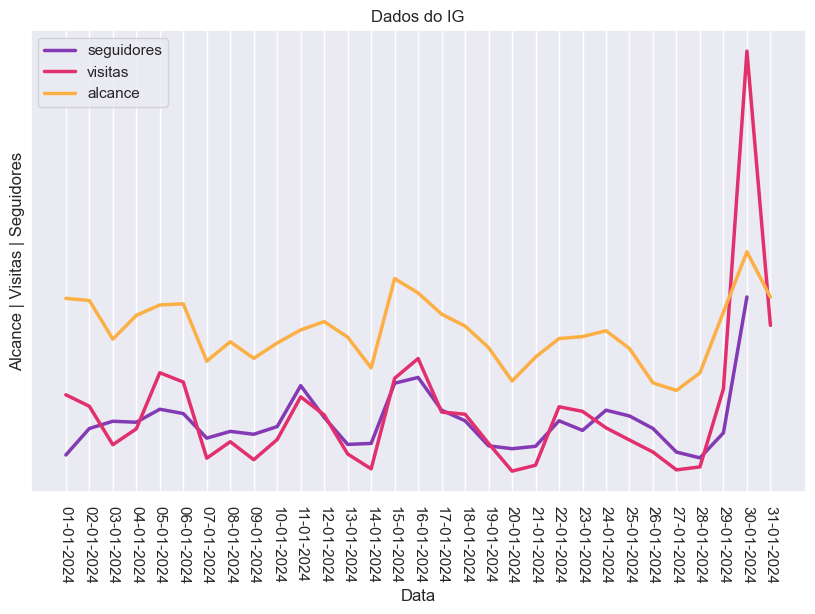
\includegraphics[width=1\textwidth]{C:/Users/Usuario/Desktop/Nova pasta/dadosIG.png}%
\end{figure}

%
\newpage%
\subsection*{Análise mensal}%
\label{subsec:Anlisemensal}%
\subsubsection*{Twitter}%
\label{ssubsec:Twitter}%
\begin{minipage}{\textwidth}%
\centering%
\begin{tabular}{@{}|c|c|c|c|@{}}%
\toprule%
\multirow{3}{*}{Mês}&Novos seguidores&Impressões&Engajamentos\\%
&\begin{footnotesize}%
variação em relação ao%
\end{footnotesize}&\begin{footnotesize}%
variação em relação ao%
\end{footnotesize}&\begin{footnotesize}%
variação em relação ao%
\end{footnotesize}\\%
&\begin{footnotesize}%
mês anterior | mesmo mês em 2023%
\end{footnotesize}&\begin{footnotesize}%
mês anterior | mesmo mês em 2023%
\end{footnotesize}&\begin{footnotesize}%
mês anterior | mesmo mês em 2023%
\end{footnotesize}\\%
\midrule%
\multirow{2}{*}{Janeiro}&2,9 mil&455,8 mil&13,2 mil\\%
&\begin{footnotesize}%
+81,3\% | +75,8\%%
\end{footnotesize}&\begin{footnotesize}%
+6\% | {-}59\%%
\end{footnotesize}&\begin{footnotesize}%
+22,2\% | {-}26,7\%%
\end{footnotesize}\\%
\midrule%
\multirow{2}{*}{Fevereiro}&('0', 0) &('0', 0) &('0', 0) \\%
&\begin{footnotesize}%
{-}100,0\% | {-}100,0\%%
\end{footnotesize}&\begin{footnotesize}%
{-}100,0\% | {-}100,0\%%
\end{footnotesize}&\begin{footnotesize}%
{-}100,0\% | {-}100,0\%%
\end{footnotesize}\\\bottomrule%
%
\end{tabular}%
\end{minipage}%
\begin{itemize}%
\item%
Legenda:%
\begin{enumerate}[label=-]%
\item%
\textbf{Impressões:} número de vezes que os usuários viram o(s) Tweet(s);%
\item%
\textbf{Engajamentos:} número total de vezes que um usuário interagiu com o(s) Tweet(s). Isso inclui todos os cliques em qualquer lugar no Tweet como: hashtags, links, avatar, nome de usuário e expansão do Tweet, Retweets, respostas e favoritos.%
\end{enumerate}%
\end{itemize}

%
\newpage%
\section*{}%
\label{sec:}%
TW: engajamento do twitter%


\begin{figure}[H]%
\centering%
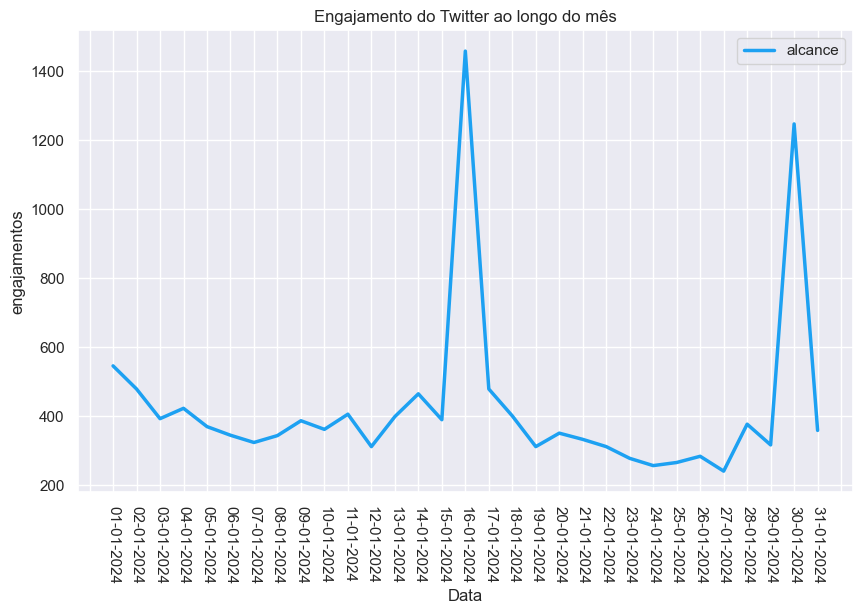
\includegraphics[width=0.45\textwidth]{C:/Users/Usuario/Desktop/Nova pasta/engajamentoTW.png}%
\end{figure}

%
\section*{}%
\label{sec:}%
TW: impressões do twitter%


\begin{figure}[H]%
\centering%
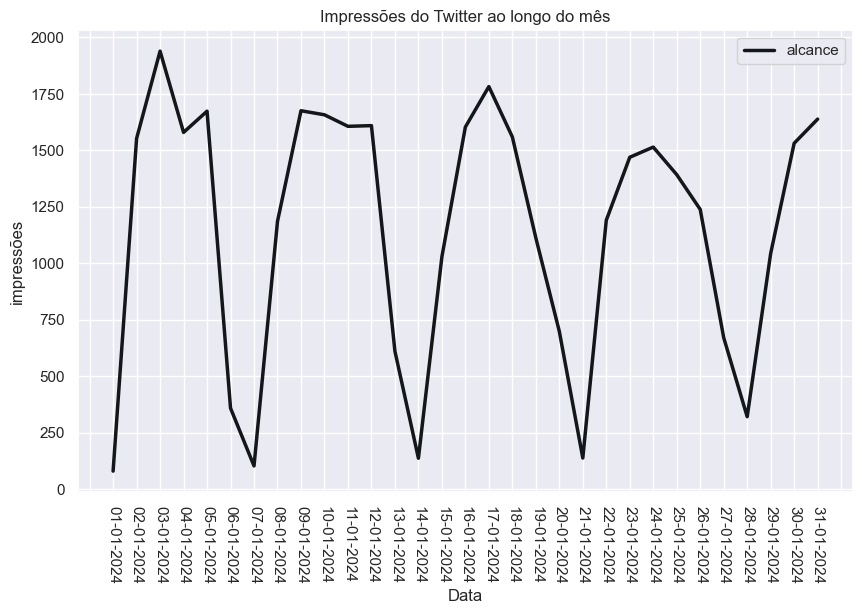
\includegraphics[width=0.45\textwidth]{C:/Users/Usuario/Desktop/Nova pasta/impressoesTW.png}%
\end{figure}

%
\section*{}%
\label{sec:}%
TW: ganho de seguidores no twitter ao logo do mês. (Esses dados levam em consideração apenas os ganhos)%


\begin{figure}[H]%
\centering%
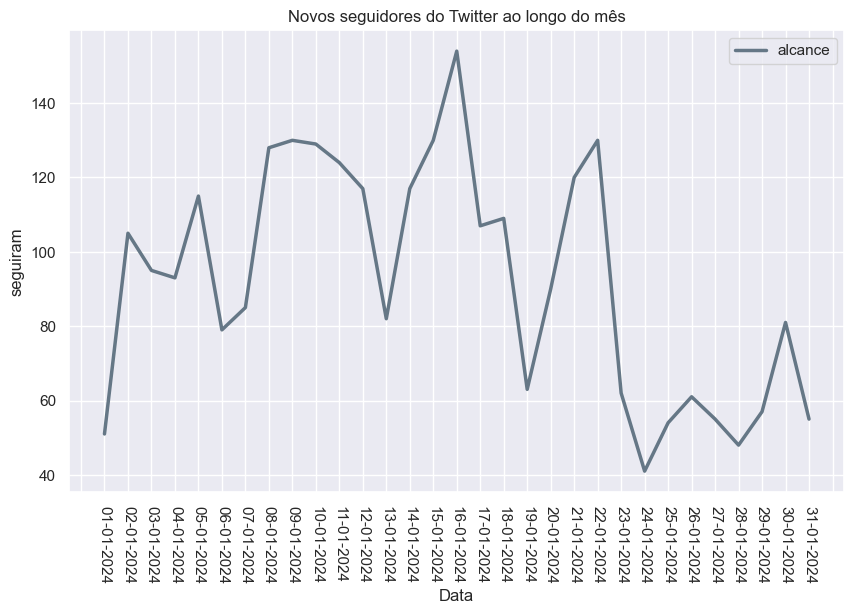
\includegraphics[width=0.45\textwidth]{C:/Users/Usuario/Desktop/Nova pasta/seguidoresTW.png}%
\end{figure}

%
\newpage%
\subsection*{Análise mensal}%
\label{subsec:Anlisemensal}%
\subsubsection*{YouTube}%
\label{ssubsec:YouTube}%
\begin{minipage}{\textwidth}%
\centering%
\begin{tabular}{@{}|c|c|c|c|@{}}%
\toprule%
\multirow{3}{*}{Mês}&Novos inscritos&Visualizações&Horas de exibição\\%
&\begin{footnotesize}%
variação em relação ao%
\end{footnotesize}&\begin{footnotesize}%
variação em relação ao%
\end{footnotesize}&\begin{footnotesize}%
variação em relação ao%
\end{footnotesize}\\%
&\begin{footnotesize}%
mês anterior | mesmo mês em 2023%
\end{footnotesize}&\begin{footnotesize}%
mês anterior | mesmo mês em 2023%
\end{footnotesize}&\begin{footnotesize}%
mês anterior | mesmo mês em 2023%
\end{footnotesize}\\%
\midrule%
\multirow{2}{*}{Janeiro}&484&132 mil&2,3 mil\\%
&\begin{footnotesize}%
+95,2\% | +389\%%
\end{footnotesize}&\begin{footnotesize}%
+95,3\% | +288\%%
\end{footnotesize}&\begin{footnotesize}%
+48\% | +172,2\%%
\end{footnotesize}\\%
\midrule%
\multirow{2}{*}{Fevereiro}&('0', 0) &('0', 0) &('0', 0) \\%
&\begin{footnotesize}%
{-}100,0\% | {-}100,0\%%
\end{footnotesize}&\begin{footnotesize}%
{-}100,0\% | {-}100,0\%%
\end{footnotesize}&\begin{footnotesize}%
{-}100,0\% | {-}100,0\%%
\end{footnotesize}\\\bottomrule%
%
\end{tabular}%
\end{minipage}

%
\section*{}%
\label{sec:}%
YouTube: visualizações por faixa etári a%


\begin{figure}[H]%
\centering%
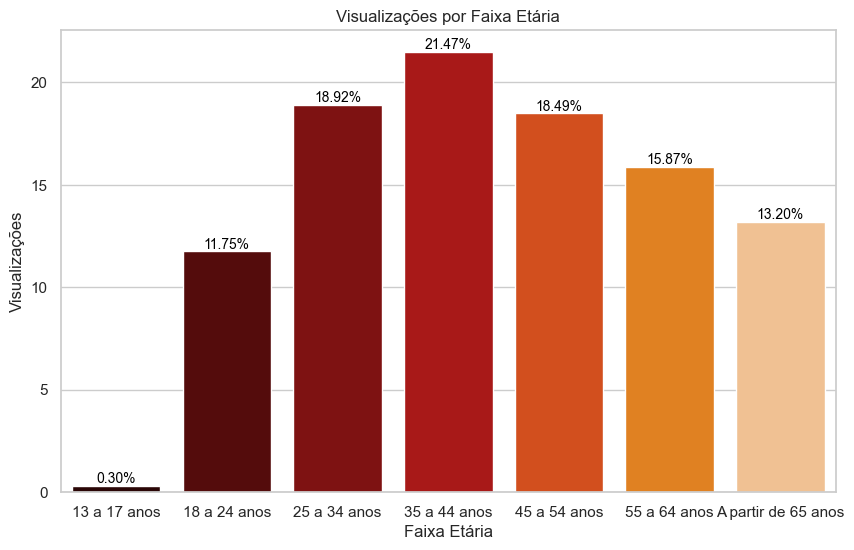
\includegraphics[width=0.7\textwidth]{C:/Users/Usuario/Desktop/Nova pasta/visualizacoesIdadeYTB.png}%
\end{figure}

%
\newpage%
\section*{}%
\label{sec:}%
YouTube: horas de exibição por faixa etária%


\begin{figure}[H]%
\centering%
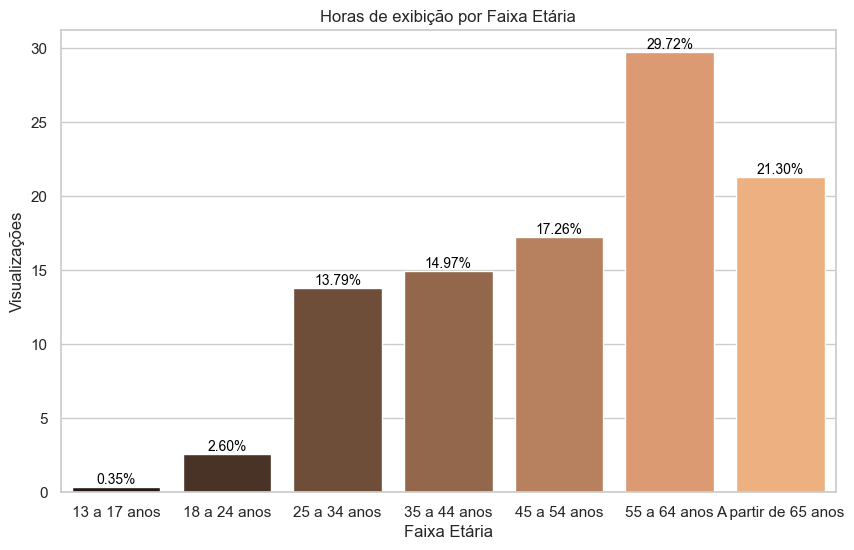
\includegraphics[width=0.7\textwidth]{C:/Users/Usuario/Desktop/Nova pasta/horasIdadeYTB.png}%
\end{figure}

%
\section*{}%
\label{sec:}%
YouTube: sexo do público%


\begin{figure}[H]%
\centering%
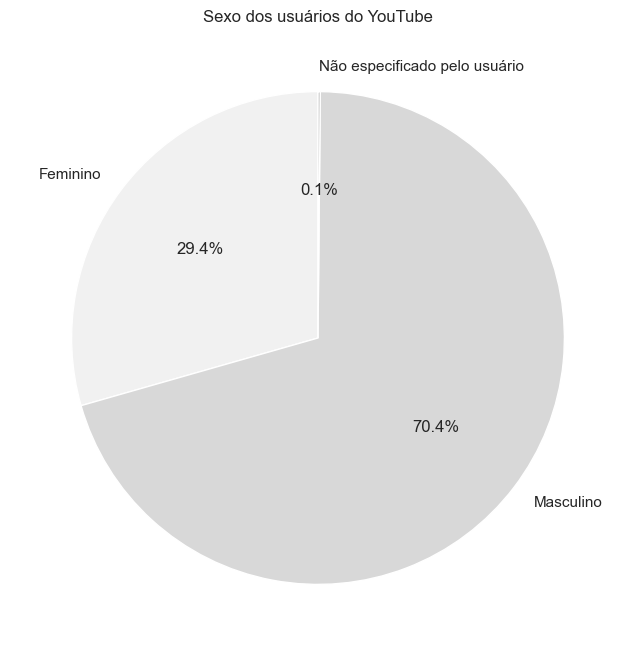
\includegraphics[width=0.6\textwidth]{C:/Users/Usuario/Desktop/Nova pasta/generoYTB.png}%
\end{figure}

%
\section*{}%
\label{sec:}%
YouTube: visualizações por cidade%


\begin{figure}[H]%
\centering%
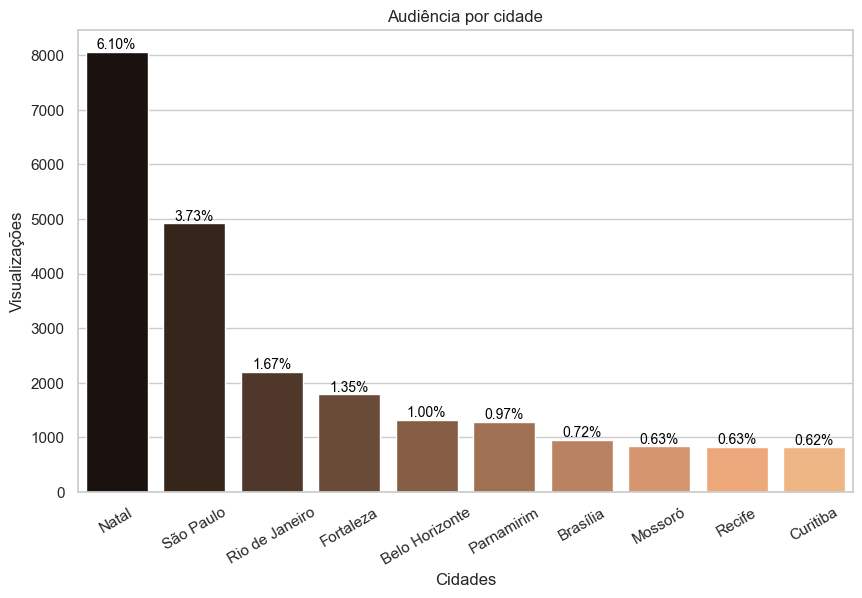
\includegraphics[width=0.7\textwidth]{C:/Users/Usuario/Desktop/Nova pasta/visualizacoesCidadeYTB.png}%
\end{figure}

%
\newpage%
\begin{itemize}%
\item%
Funcionamento dos algoritmos:%
\begin{enumerate}[label=-]%
\item%
\textbf{Facebook:} O algoritmo do Facebook prioriza os conteúdos que geram mais interações, como curtidas, comentários e compartilhamentos. Ele também considera o grau de relacionamento entre os usuários e as contas que eles seguem, mostrando mais publicações de amigos e familiares do que de páginas. Além disso, o Facebook leva em conta a relevância e a atualidade dos conteúdos, dando mais destaque para as notícias e os assuntos do momento;%
\item%
\textbf{Instagram:} O a lgoritmo do Instagram também se baseia no engajamento, no relacionamento e na temporalidade dos conteúdos. Ele mostra primeiro as postagens e as histórias das contas com as quais o usuário mais interage, seja por meio de curtidas, comentários, mensagens diretas ou buscas. Ele também valoriza os conteúdos mais recentes e mais relevantes para o usuário, de acordo com os seus interesses e hábitos;%
\item%
\textbf{Twitter:} O algoritmo do Twitter tem duas formas de exibir os conteúdos: o modo cronológico e o modo destacado. No modo cronológico, o usuário vê os tweets mais recentes em ordem de publicação. No modo destacado, o usuário vê os tweets mais relevantes para ele, de acordo com o seu perfil, as suas interações e os assuntos do momento. O Twitter também mostra os tweets mais populares e mais comentados na seção “O que está acontecendo”;%
\item%
\textbf{YouTube:} O algoritmo do YouTube tem como objetivo aumentar o tempo de permanência dos usuários na plataforma, recomendando os vídeos que eles têm mais chances de assistir e se engajar. Para isso, ele considera fatores como o histórico de visualização, as preferências, as inscrições, a localização e o feedback dos usuários. Ele também leva em conta a qualidade e a relevância dos vídeos, analisando aspectos como o título, descrição, tags, miniaturas e os metadados.%
\end{enumerate}%
\end{itemize}%
\newpage%
\begin{minipage}{\textwidth}%
\centering%
\begin{large}%
Observações%
\end{large}%
\end{minipage}%
\begin{itemize}%
\item%
Sessões:%
\begin{enumerate}[label=-]%
\item%
Por padrão, a sessão é encerrada após 30 minutos de inatividade, mas é possível ajustar esse limite para que ela dure de alguns segundos a várias horas.%
\end{enumerate}%
\begin{enumerate}[label=]%
\item%
O Google Analytics começa a contar a partir do momento em que um usuário acessa seu site. Se depois de 30 minutos este usuário não fizer uma interação, a sessão é finalizada. No entanto, toda vez que ocorre uma interação com um elemento (como um evento, interação de rede social ou uma nova página), o Google Analytics reinicia o tempo de vencimento adicionando 30 minutos a partir do momento da interação.
 Um único usuário pode abrir várias sessões. Essas sessões podem ocorrer no mesmo dia ou em vários dias, semanas ou meses. Assim que uma sessão termina, existe a oportunidade de iniciar uma nova sessão. Há dois métodos para o encerramento de uma sessão:%
\end{enumerate}%
\begin{enumerate}[label=]%
\item%
Um único usuário pode abrir várias sessões. Essas sessões podem ocorrer no mesmo dia ou em vários dias, semanas ou meses. Assim que uma sessão termina, existe a oportunidade de iniciar uma nova sessão. Há dois métodos para o encerramento de uma sessão:%
\begin{enumerate}[label=•]%
\item%
Vencimento por tempo:%
\begin{enumerate}[label=•]%
\item%
Depois de 30 minutos de inatividade;%
\item%
À meia-noite.%
\end{enumerate}%
\end{enumerate}%
\begin{enumerate}[label=•]%
\item%
Mudança de campanha::%
\begin{enumerate}[label=•]%
\item%
Se um usuário entra por uma campanha, sai e depois volta para outra. (Fecha o site e entra novamente, por exemplo).%
\end{enumerate}%
\end{enumerate}%
\end{enumerate}%
\end{itemize}%
\begin{itemize}%
\item%
Calculos de porcentagem:%
\begin{enumerate}[label=-]%
\item%
\textbf{Variação:} \Large{\left\(\frac{Mês\ Atual\ -\ Mês\ Anterior}{|Mês\ Anterior|}\right\)}\normalsize * 100.%
\end{enumerate}%
\begin{enumerate}[label=]%
\item%
O cálculo é feito dessa forma pois quero saber  qual a diferença, em porcentagem, do valor atual em relação ao anterior, seja esse valor anterior o do mês passado ou o do mesmo mês no ano passado. Em outras palavras, quero saber o quanto o valor do mês atual cresceu ou diminuiu em ralação ao outro.%
\item%
Caso a variação do mês atual com o anterior seja de +10,6\%, além da constatação óbvia de que é um número 10,6\% maior, também quer dizer que essa porcentagem equivale a 10,6\% do valor do mês anterior. Ou seja, se somarmos o valor equivalente a essa porcentagem ao mês anterior o resultado será o valor do mês atual (ou pelo menos algo MUITO próximo).%
\item%
Por exemplo: se no mês atual o portal teve 957 novos seguidores e o anterior 586, isso quer dizer que o mês atual teve aumento de,  aproxiamdamente, 63,33\%. E sabendo que 63,33\% de 586 é, aproximadamente, 371, podemos provar que 957 - 371 = 586 ou que 586 + 371 = 957.%
\end{enumerate}%
\begin{enumerate}[label=-]%
\item%
\textbf{Taxa de fixação:} \Large{\left\(\frac{Total\ de\ novos\ seg.\ no\ mês\ -\ Total\ de\ seg.\ perdidos\ no\ mês}{Total\ de\ novos\ seg.\ no\ mês}\right\)}\normalsize * 100.%
\end{enumerate}%
\begin{enumerate}[label=]%
\item%
Nesse cálculo eu quero saber quantos por cento do total de seguidores ganhos continuaram seguindo a rede social em questão.%
\item%
É importante obeservar que as pessoas que deixaram de seguir não fazem parte apenas dos mesmos que seguiram durante o mês analisado (caso o cálculo ou o texto passem essa impressão), ou apenas dos usuários que já seguiam antes. E saber de qual grupo faz parte a pessoa que deixou de seguir é um dado que não é possível de se obter.%
\end{enumerate}%
\end{itemize}%
\end{document}